%%%%%%%%%%%%%%%%%%%%%%%%%%%%%%%%%%%%%%%%%
% Journal Article
% LaTeX Template
% Version 1.3 (9/9/13)
%
% This template has been downloaded from:
% http://www.LaTeXTemplates.com
%
% Original author:
% Frits Wenneker (http://www.howtotex.com)
%
% License:
% CC BY-NC-SA 3.0 (http://creativecommons.org/licenses/by-nc-sa/3.0/)
%
%%%%%%%%%%%%%%%%%%%%%%%%%%%%%%%%%%%%%%%%%

%----------------------------------------------------------------------------------------
%	PACKAGES AND OTHER DOCUMENT CONFIGURATIONS
%----------------------------------------------------------------------------------------

\documentclass{article}

%\documentclass{aastex}  % version 5.0 or prior
%\usepackage{natbib}



\usepackage{graphicx}
\usepackage{lipsum} % Package to generate dummy text throughout this template
%\usepackage[sc]{mathpazo} % Use the Palatino font
\usepackage[T1]{fontenc} % Use 8-bit encoding that has 256 glyphs
\linespread{1.05} % Line spacing - Palatino needs more space between lines
\usepackage{microtype} % Slightly tweak font spacing for aesthetics

\usepackage[margin=1in,columnsep=20pt]{geometry} % Document margins
\usepackage{multicol} % Used for the two-column layout of the document
\usepackage[hang, small,labelfont=bf,up,textfont=it,up]{caption} % Custom captions under/above floats in tables or figures
\usepackage{booktabs} % Horizontal rules in tables
\usepackage{float} % Required for tables and figures in the multi-column environment - they need to be placed in specific locations with the [H] (e.g. \begin{table}[H])
\usepackage{hyperref} % For hyperlinks in the PDF
\usepackage{subcaption}

\usepackage{lettrine} % The lettrine is the first enlarged letter at the beginning of the text
\usepackage{paralist} % Used for the compactitem environment which makes bullet points with less space between them
\usepackage{amsmath}
\usepackage{abstract} % Allows abstract customization
\renewcommand{\abstractnamefont}{\normalfont\bfseries} % Set the "Abstract" text to bold
\renewcommand{\abstracttextfont}{\normalfont\small\itshape} % Set the abstract itself to small italic text

\usepackage{titlesec} % Allows customization of titles
%\renewcommand\thesection{\Roman{section}} % Roman numerals for the sections
%\renewcommand\thesubsection{\Roman{subsection}} % Roman numerals for subsections
%\renewcommand\thesubsubsection{\Alph{subsubsection}} % Roman numerals for subsections
\titleformat{\section}[block]{\LARGE\scshape}{\thesection}{1em}{} % Change the look of the section titles
\titleformat{\subsection}[block]{\Large\scshape}{\thesubsection}{1em}{} % Change the look of the section titles
\titleformat{\subsubsection}[block]{\large\scshape}{\thesubsubsection}{1em}{} % Change the look of the section titles

\usepackage{fancyhdr} % Headers and footers
\pagestyle{fancy} % All pages have headers and footers
\fancyhead{} % Blank out the default header
\fancyfoot{} % Blank out the default footer
\fancyhead[C]{Montana State University \quad $\bullet$ \quad CSCI 466 Artificial Intelligence \quad $\bullet$ \quad Group 21} % Custom header text
\fancyfoot[RO,LE]{\thepage} % Custom footer text

\newcommand{\ve}[1]{\boldsymbol{\mathbf{#1}}}

\title{\vspace{-15mm}\fontsize{24pt}{10pt}\selectfont\textbf{CSCI 446 Artificial Intelligence \\[2mm] Project 3 Design Report} } % Article title
\date{\today}
\author{
\large
\textsc{Roy Smart} \and \textsc{Nevin Leh} \and \textsc{Brian Marsh}\\[2mm] % Your name
}


%----------------------------------------------------------------------------------------

\begin{document}

	\maketitle % Insert title
	\thispagestyle{fancy} % All pages have headers and footers
	\normalsize

	\section{Introduction}
	Introduce Machine Learning Algorithm (MLA)!!!!
	Explain classification problem!!!
	\section{Datasets}
		\subsection{Dataset Representation}
			We will define a \textit{datum} to be a vector consisting of the class as the zeroth element and the associated attributes as the rest of the elements. Classes and attributes will be represented by an integer. Continuous data will be binned before it is inserted into each datum. The resolution of the bins will be a variable that will have to be tuned. Each dataset will be represented as a vector of datums.
		\subsection{Data Imputation}
			Imputation is the process of approximating missing values in the datasets. 
			To our knowledge there is only one dataset that has real missing values: the Wisconsin Breast Cancer Database. 
			The 1984 United States Congressional Voting Records Database appears to have missing values, but these can actually be interpreted as a stance on a particular issue. 
			Since the breast cancer database has a small proportion of missing values, it is appropriate to simply eliminate datums with missing values. 
			The authors assert that trying to train a MLA with imputed values would only create unnecessary bias in the network.
			
			However, it is a common real-world problem to attempt to classify an unknown, incomplete datum, therefore we will perform imputation on the validation datasets. 
			To approximate the missing values we will first try a hot-deck imputation, where missing attribute values of a given datum are constructed by selecting a random member of that datum's class and copying the value of the attribute. 
			If the hot-deck is unsuccessful, we will attempt to fill in the missing values using a regression model developed in \textit{Mathematica}.
		\subsection{Cross-validation}
			\label{cv}
			To partition the full datasets into test and training datasets, we will use 10-fold cross validation. 
			This method partitions the data into ten \textit{folds} and uses one fold for testing data and the remaining nine folds for the training dataset. 
			This process is repeated nine more times until every fold has been used as a test dataset. 
			We selected this method because it will allow the convergence measurement described in Section \ref{convergence} to be applied over a larger range, which allows us to measure the rate of convergence for each MLA more accurately.
	\section{Machine Learning Algorithms}
		\label{mla}
		\subsection{$k$-Nearest Neighbors}
		\subsection{Naive Bayes}
			\label{nbw}
			\subsubsection{Description}
				\label{nb_des}
				\textit{Naive Bayes} uses the principle of Bayesian learning to solve the classification problem. This algorithm is said to be naive because it considers the attributes to be conditionally independent when performing classifications. Under this scheme, the probability distribution of each class $C$ is given the set of attributes $x_1,...,x_n$ is written by \cite{ai} as
				\begin{equation}					
					\ve{P}(C|x_1,...,x_n) = \alpha \ve{P}(C) \prod_i \ve{P}(x_i| C) \label{nb_pd}
				\end{equation}
				where, using the maximum likelihood hypothesis, $\ve{P}(C)$ prior probability of the class $C$ in the training dataset, $\ve{P}(x_i|C)$ is the likelihood of attribute $x_i$ given $C$, and $\alpha$ is a normalization constant. To find $\ve{P}(C)$ the we simply say it is equal to the proportion of $C$ observed in the training dataset. Likewise we can calculate the likelihood using
				\begin{equation*}
					P(a|b) = \frac{P(a \land b)}{P(b)}
				\end{equation*}
				where the probabilities are calculated using the number of occurrences in the training dataset. So, using equation \ref{nb_pd} we can calculate the probability of a particular set of attributes being classified as class $C$. Then, we simply select the class with the largest probability for our prediction. In this way, naive Bayes can make predictions using only the probability ratios constructed from the training dataset. The probability distribution in the naive Bayes algorithm can be viewed as a Bayesian network, shown in Figure \ref{nb} where each attribute is only connected to the class, and there are no relationships between attributes.
				\begin{figure}[h]
					\centering
					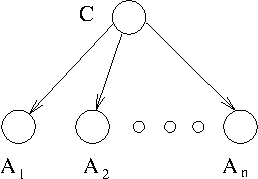
\includegraphics[width=0.3\textwidth]{fig/nb}
					\caption{An example of a Bayesian network for naive Bayes. The root $C$ is the class, the leaves $A_1,...,A_n$ are the attributes \cite{Friedman1997}}
					\label{nb}
				\end{figure}
			\subsubsection{Design Implications}
				This algorithm should be very straightforward to implement. During the training phase, we simply loop through the dataset and tally how many times each class takes on every value of each attribute. During the testing phase, the algorithm uses the equations described in Section \ref{nb_des} to select the most probable class.
		\subsection{TAN}
			\subsubsection{Description}
				\textit{Tree-Augmented Naive Bayes} (TAN) is an extension to the naive Bayes algorithm described in Section \ref{nbw}. First described by \cite{Friedman1997} TAN relaxes the assumption that the attributes are conditionally independent and allows each attribute to depend on only one other attribute. It accomplishes this by constructing a fully-connected, undirected graph out of the attributes in the Bayesian network for the naive Bayes algorithm (Figure \ref{nb}). TAN then assigns a weight to each connection in the graph using the \textit{mutual information function}, given by
				\begin{equation*}
					I_P(\ve{X};\ve{Y}) = \sum_{\ve{x},\ve{y}} P(\ve{x},\ve{y}) \log \left( \frac{P(\ve{x},\ve{y})}{P(\ve{x})P(\ve{y})} \right).
				\end{equation*}
				Applying the this weight to the edges allows us to construct a minimum spanning tree of the graph. We can then make the spanning tree directed by choosing a root node and setting the direction of all edges to be outward from it. The result is exemplified in Figure \ref{tan}.
				\begin{figure}[h]
					\centering
					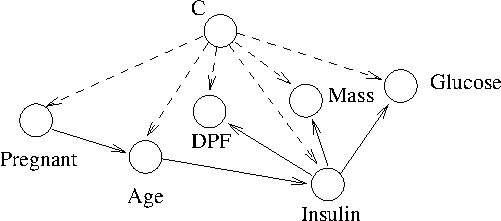
\includegraphics{fig/tan}
					\caption{An example of the directed minimum spanning tree produced by TAN. Dashed lines represent the original naive Bayes representation and the solid lines represent the spanning tree \cite{Friedman1997}.}
					\label{tan}
				\end{figure}
				Using this representation, we can calculate the analog of equation \ref{nb_pd}, the probability distribution using the expression given by \cite{Zheng2010}
				\begin{equation}
						\ve{P}(C|x_1,...,x_n) = \alpha \ve{P}(C) \prod_i \ve{P}(x_i| C, \pi(x_i)) \label{tan_pd}
				\end{equation}
				where $\pi(x_i)$ is the parent of the attribute $x_i$ in the directed minimum spanning tree. Then, using a similar process to that described in Section \ref{nbw} we can classify a set of attributes by selecting the class with the highest probability calculated from equation \ref{tan_pd}.
			\subsubsection{Design Implications}
				To develop the TAN algorithm, we will need to implement a tree structure to represent the naive Bayesian network and the associated minimum spanning tree. To find the minimum spanning tree we will need an implementation of Prim's algorithm. If appropriate we will use the implementation of Prim's algorithm provided in the Boost C++ libraries, otherwise we will develop our own implementation of Prim's algorithm. Once the minimum spanning tree is constructed we can appropriate the probability calculations developed for naive Bayes to calculate the value of equation \ref{tan_pd} for classification.
		\subsection{ID3}
			\subsubsection{Description}
				\textit{Iterative Dichotomiser 3} (ID3) is an algorithm that creates a decision tree and uses it to make inductive inferences about a set of data.
				The decision tree approach to making these inferences is a fairly obvious one.
				Make a decision tree that correctly classifies all the individuals in the training data.
				Since the goal of this solution is to generalize classification, it makes sense to use the smallest tree that can still correctly classify all of the training data.
				The naive way of finding the shortest tree would be to generate all possible trees and select the shortest one according to\cite{Quinlan1986}.
				The problem that one encounters is the very large, but finite, number of decision trees that are capable of correctly classifying all data.
				The computation required to do this is unfeasible large.
				ID3 provides a good, but not optimal, solution to this problem.
		
				ID3 is an iterative process that generates a short tree by splitting the tree one attribute at a time. The first attribute to be used is the one with the most information gain. Information gain can described as how much entropy the system lost by splitting on an attribute. The equation for entropy is as follows:
				\begin{equation*}
					H(S) = \sum_{i=1}^{n} \left( -p_i \log_2 p_i \right).
				\end{equation*}		
				
				where $p_i$ is the proportion of the number of datums in class $i$ to the total number of datums in the set $S$. To use this equation the entropy of the whole system is determined first. Then the sum of the entropy for each branch is calculated and subtracted from the total entropy. The goal is to maximize this difference so the tree will be small and more general.
				
				The rest of the algorithm is just iterating through as the tree is made and redo the calculation on an attribute that has not been split yet. The tree is finished when all leaf nodes are a single class or when attributes to split on have run out. In this case each leaf node that does not have a class is assigned the most common class in that leaf.
				
				One bias that ID3 introduces is the fact that attributes that have a large amount of possibilities will naturally have a higher gain and, therefore, will be chosen first. To combat this we will use gain ratio instead. Gain ratio takes into account the number of possibilities for each algorithm.
				
				Another problem is that the tree still might not be general enough and could be trimmed down further. To help with this we will implement reduced error pruning. The general idea is to fully create a tree and then prune branches while checking if the missing branch still results in the same classification for the pruning set. The pruning set is a subset of the of the training set that is not used in the normal training process.
			\subsubsection{Design Implications}
				This algorithm will affect the structure of our code greatly. A tree structure will have to be created that can contain subsets of the training set and also leaf values for when a classification is found. In addition the training set is going to have to be divided to get a validation set to perform reduced error pruning. The main body of the learning part of the algorithm will be in a while loop with the conditions above. The search part of the algorithm will just consist of transversing the tree according to the attributes belonging to the query.
	\section{Software Architecture}
		To reliably compare the four machine learning algorithms on five different datasets, we will use inheritance and C++ virtual classes that allows us to perform algorithm- and dataset-independent analyses on the MLAs. The inheritance structure is described in Figure \ref{uml}.
		\begin{figure}[h]
			\centering
			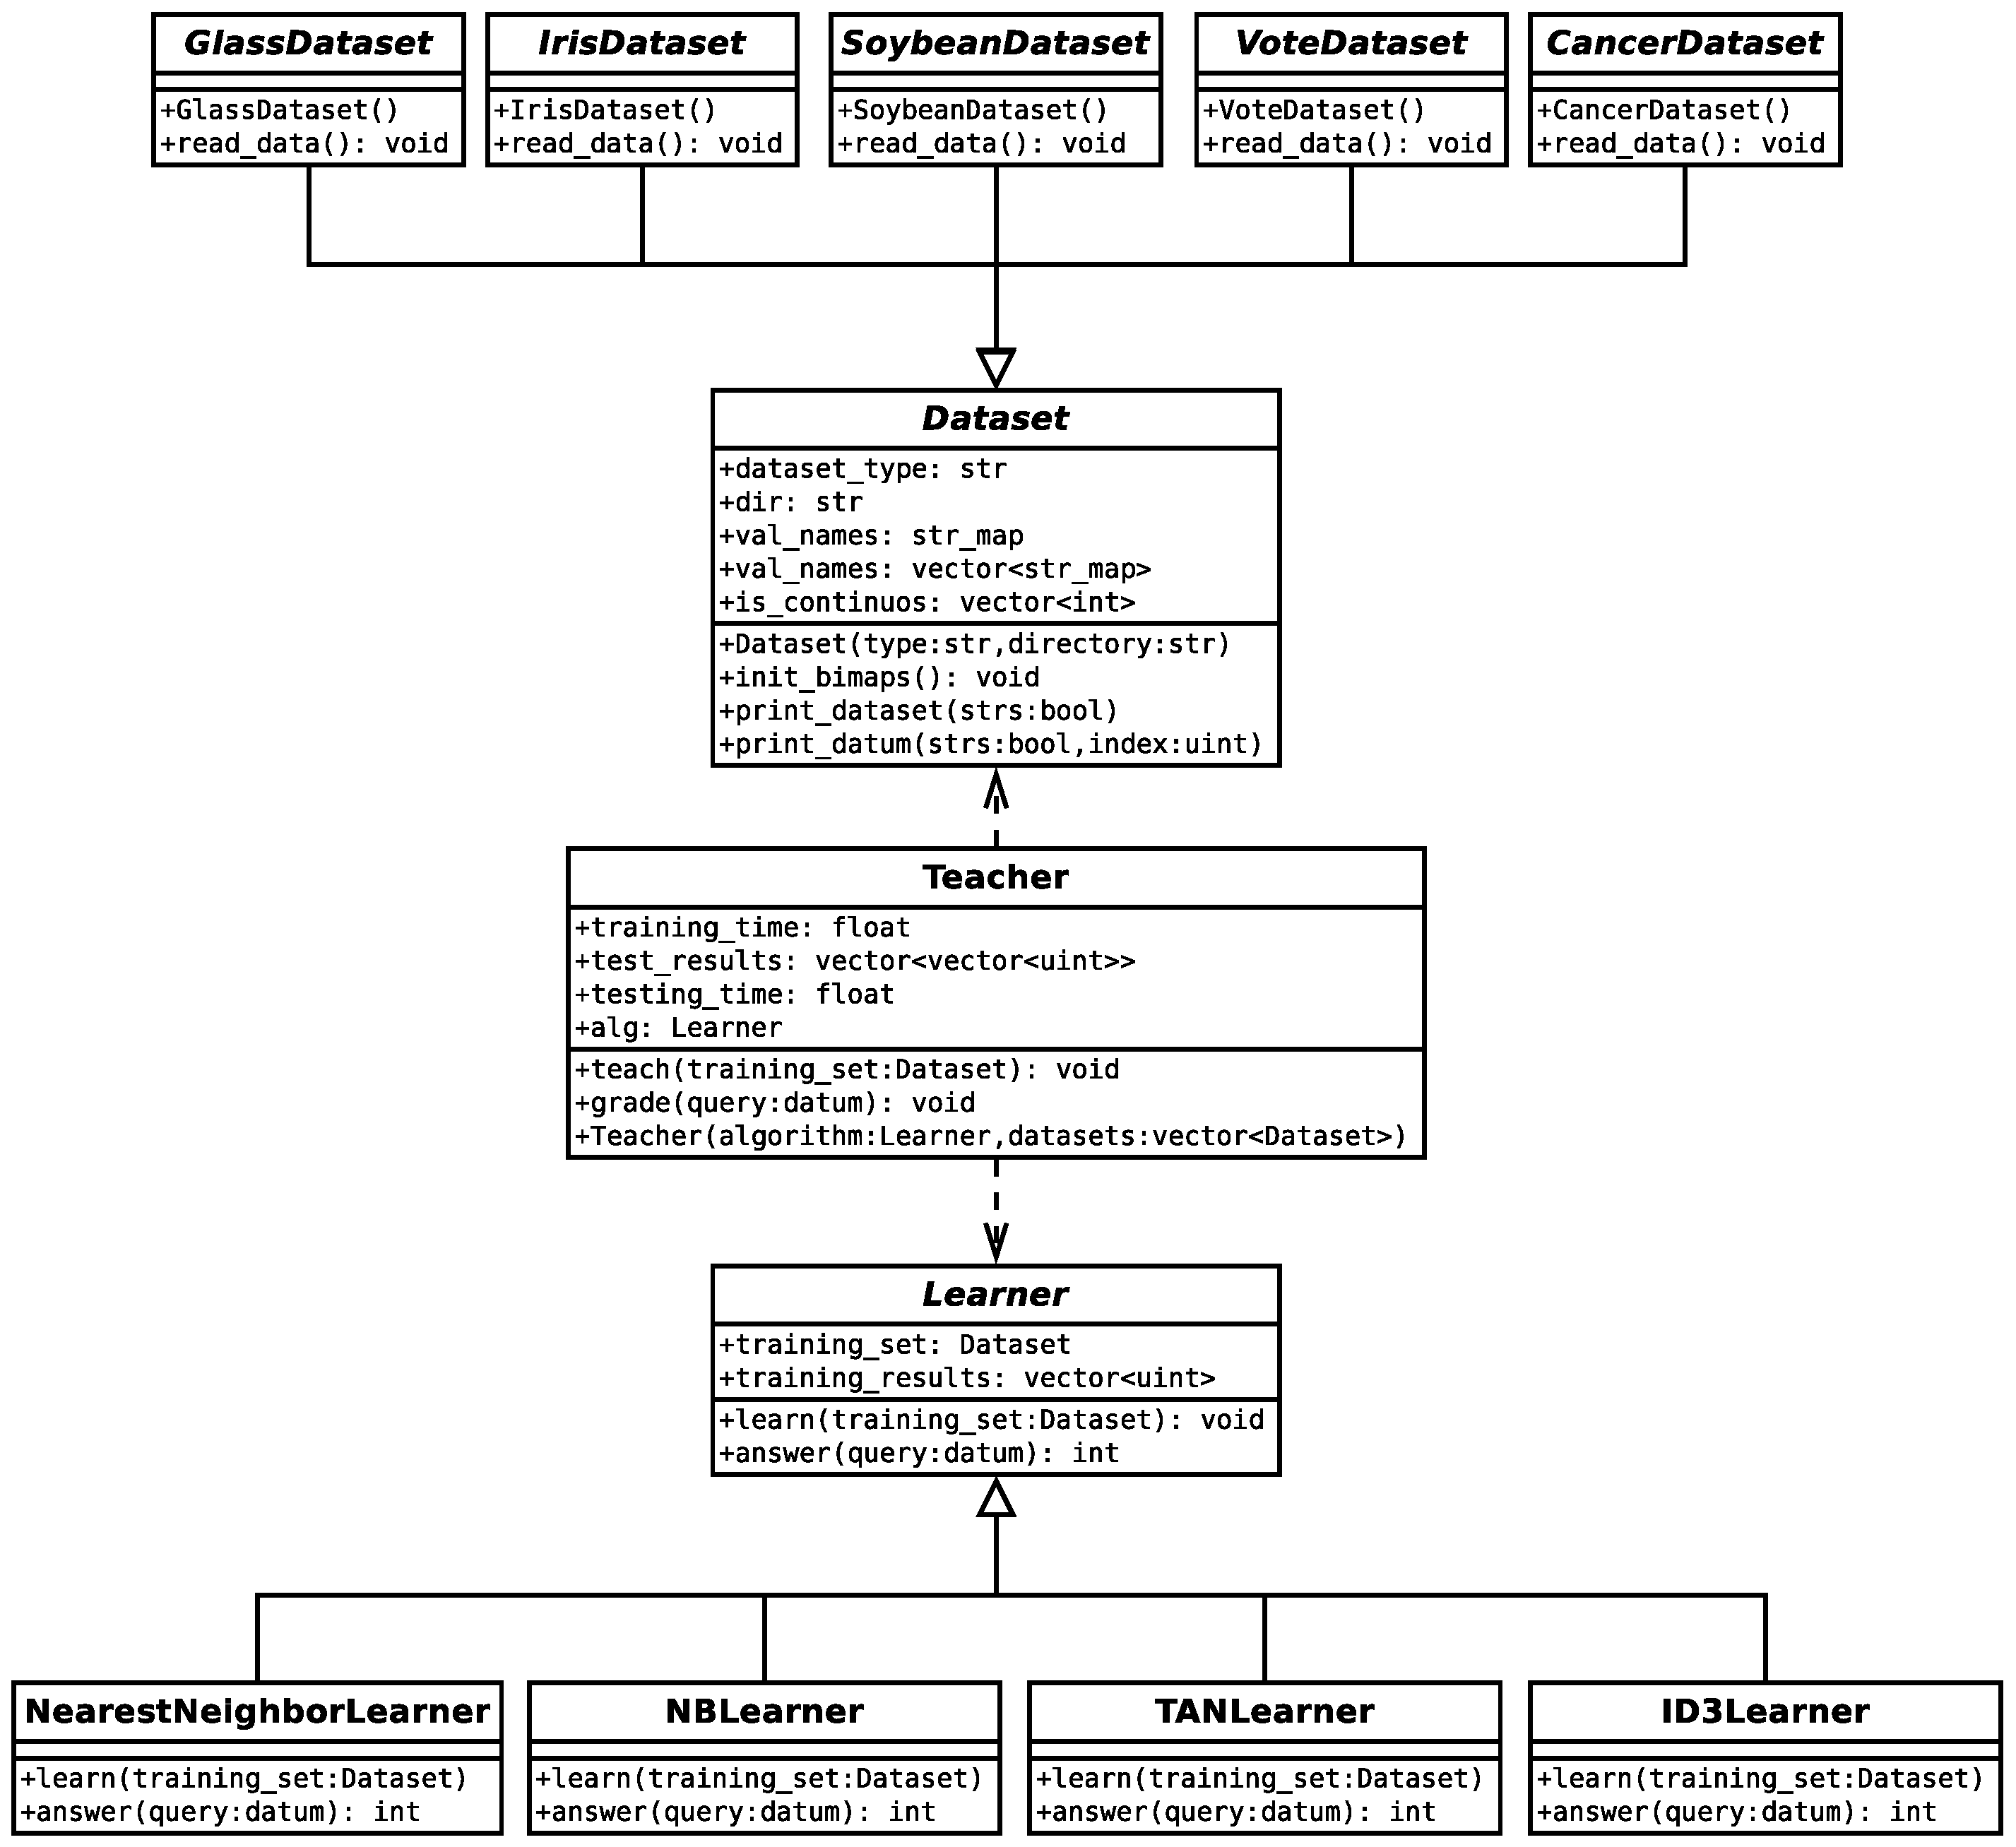
\includegraphics[width=0.5\textwidth]{fig/UML_Design}
			\caption{A high-level description of the program architecture in UML.}
			\label{uml}
		\end{figure}	
		Each of the datasets will be encapsulated in an associated class, e.g. the Glass Identification Database will be stored in a class denoted \texttt{GlassDataset}. This class will inherit from the virtual class \texttt{Dataset}, which defines a dataset as a vector of integers, and also a set of associated functions for selected subsets of the dataset, printing the dataset, etc.
		
		We will also implement a virtual class called \texttt{Learner}, which operates on a single training dataset. \texttt{Learner} defines the two functions \texttt{learn()} and \texttt{answer()} which will be used to perform training and testing respectively. Therefore, each of the four MLAs will inherit from learner and implement the two functions \texttt{learn()} and \texttt{answer()} based on the algorithm descriptions in Section \ref{mla}. 
		
		To relate MLAs to datasets, we will define a \texttt{Teacher} class that is responsible for training and validating the MLAs, and measuring their performance. This class will also be responsible for performing the convergence measurement described in Section \ref{convergence}.
		
		Not depicted in Figure \ref{uml} is a class called \texttt{Validation}. This class will be responsible for the 10-fold cross validation described in Section \ref{cv}. \texttt{Validation} will partition the datasets into training and testing datasets and provide them to the \texttt{Teacher} to train and validate the MLAs.
	\section{Experiment Design}
		\subsection{Algorithm Accuracy}
			\subsubsection{Precision}
			Precision is the proportion of results that are relevant according to \cite{ai}. This is better described as the fraction of the number of correct classifications for a class and the total amount of datums that were classified as that class. This process will have to be done one class at a time and then averaged.
			This is a good metric to look at because it tells you the proportion of correct classifications to all classifications. To do this we will have to save the true positive, false positive, true negative, and false negative counts for each class as validation occurs.
			\subsubsection{Recall}
			Recall is the proportion of relevant datums that that are correctly classified. This is better described as the fraction of the number of correct classifications for a class and the total number of datums that should have been classified as that class. This metric seems similar to precision but is useful because it tells you the proportion of correct classifications to the actual number of datums in that class. In essence it tells you how many classifications you missed rather than how many were correct. Again the process will have to be done one class at a time and then averaged. 
		\subsection{Algorithm Time-Complexity}
		For algorithm time complexity we will use a simple timer to get an estimation of the run time. Since a timer sometimes is not necessarily a good metric for time-complexity we will also attempt to determine the time complexity by inspection of each algorithm.
		\subsection{Algorithm Convergence}
			\label{convergence}
		Algorithm Convergence is a metric that shows how well the algorithm performs with different amounts of training data. The idea is to incrementally add data to the training set and see how well validation performs at each increment. This is an interesting metric to have because it gives us an indication as to how much training data is needed for each algorithm. This will add a step to our validation process since we will have to validate every time we increment the amount of training data.


	%\bibliographystyle{apj}
	\bibliographystyle{apalike}	
	\bibliography{sources}
\end{document}
